%%% Local Variables:
%%% mode: latex
%%% TeX-master: t
%%% End:

\subsection{Development Methodology}

In this project we use both waterfall and scrum methodologies.
We used the waterfall methodology for developing the smart contract because we can not update it once we deploy it. And for the rest, we used the scrum methodology.

Scrum, is a framework for project management, with an initial emphasis on software development, although it has been used in other fields including research, sales, marketing and advanced technologies. It is designed for teams of ten or fewer members, who break their work into goals that can be completed within time-boxed iterations, called sprints, no longer than one month and most commonly two weeks. The scrum team assesses progress in time-boxed daily meetings of 15 minutes or fewer, called daily scrums (a form of stand-up meeting). At the end of the sprint, the team holds two further meetings: the sprint review which demonstrates the work done to stakeholders to elicit feedback, and sprint retrospective which enables the team to reflect and improve.

\namedfigure
{!htbp}
{img:scrum}
{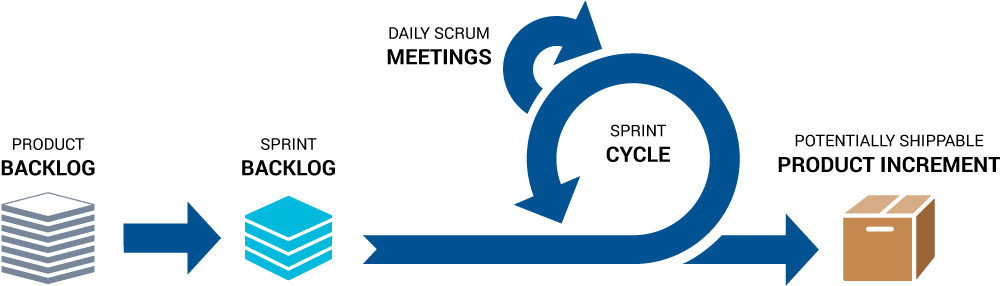
\includegraphics[width=\textwidth]{scrum.png}}
{Agile scrum development process.}
